% Chapter Template

\chapter{Results} % Main chapter title

\label{chap:results} 
This chapter will summarize the results of this work. First, the results of simulating the susceptible population (\B{S})
in the region of Hesse will be presented. Then the results of a sensitivity analysis for the variables $\alpha$ and
$q$ will be shown. These are the two variables that are governing the transition from \B{S} to
the Exposed (\B{E}) group ($\alpha$ variable) and transition form \B{E} to the Infected (\B{I}) group ($q$ variable).


%----------------------------------------------------------------------------------------
%	SECTION 1
%----------------------------------------------------------------------------------------

\section{Simulating the susceptible population of Hesse}
\label{sec:sim_res}
During this work we simulated the susceptible population of Hesse. 26 regions were simulated over a time period of
76, 60 and 50 days respectively. We will show both the absolute and percentage difference between the simulated
and the original data for each time frame.\newline

One challenge of this project was the visualization of the obtained results. Since the number of susceptible
individuals that resign in this group is much greater than the number individuals that transition to the exposed state,
changes in this group are difficult to observe. Because of this we decided against comparing simulated and real world
\B{S} data directly. We instead  calculated and compared the number of individuals that
transitioned from \B{S} to \B{E}. This was done by subtracting the number of susceptible individuals at data point \I{t=x} from
the starting point \I{t=0}. The result is the cumulative change of susceptibles at any given time point, which is equivalent to the 
sum of all exposed individuals at any given time. These results are much easier to visualize, compare and understand.
\textcolor{red}{ADD OPTIMAL VALUES FOR $\alpha$ AND $q$!! Add set values for other variables to methods!}

%-----------------------------------
%	SUBSECTION 1
%-----------------------------------
\subsection{Simulation trends and trend changes with fewer data points}
We first investigated the trends of the \B{S} group in order to get a general understanding for the accuracy of the simulated
data. For this purpose each region was investigated by comparing simulation results and real world data in a graph.
\hyperref[fig:76_sim_expl]{Figure \ref*{fig:76_sim_expl}} shows three exemplary regions with 76, 60 and 50 simulated data
points respectively. The regions were chosen based on their general trends and are examples for regions with a positive deviation
(to many transition events), a negative deviation (to few transition events) and a generally similar trend.\newline

\begin{figure}[h]
	\centering
	\begin{subfigure}[b]{0.3\textwidth}
		\centering
		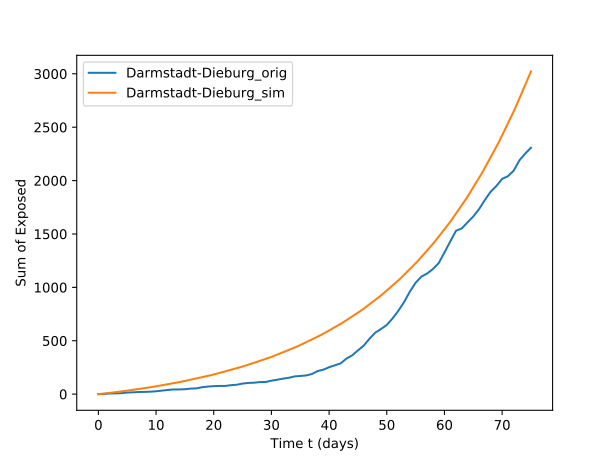
\includegraphics[width=\textwidth]{./figures/76d/24_Darmstadt-Dieburg.png}	
		\caption{}
	\end{subfigure}
	\hfill
	\begin{subfigure}[b]{0.3\textwidth}
		\centering
		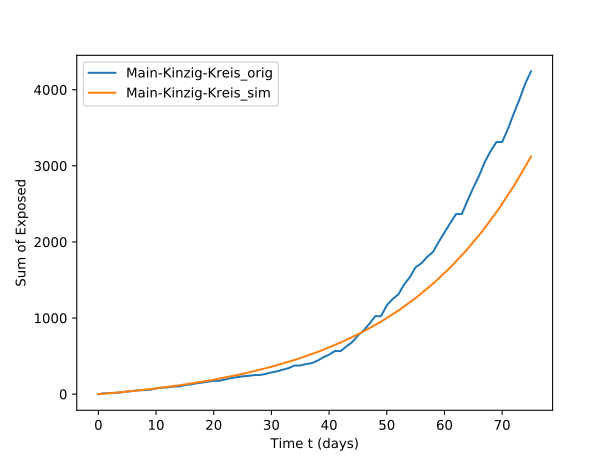
\includegraphics[width=\textwidth]{./figures/76d/13_Main-Kinzig-Kreis.png}	
		\caption{}
	\end{subfigure}
	\hfill
	\begin{subfigure}[b]{0.3\textwidth}
		\centering
		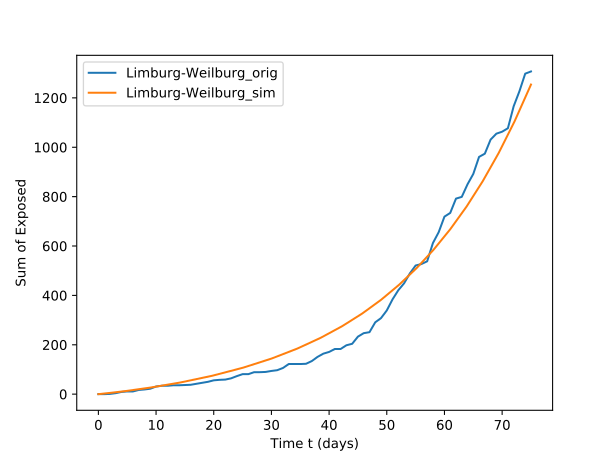
\includegraphics[width=\textwidth]{./figures/76d/10_Limburg-Weilburg.png}	
		\caption{}
	\end{subfigure}
	\begin{subfigure}[b]{0.3\textwidth}
		\centering
		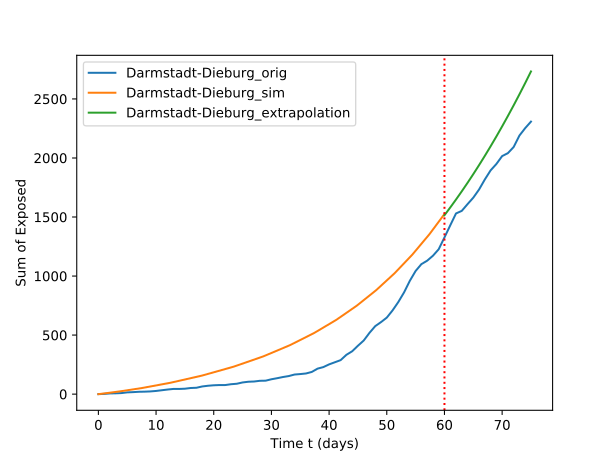
\includegraphics[width=\textwidth]{./figures/60d/24_Darmstadt-Dieburg.png}	
		\caption{}
	\end{subfigure}
	\hfill
	\begin{subfigure}[b]{0.3\textwidth}
		\centering
		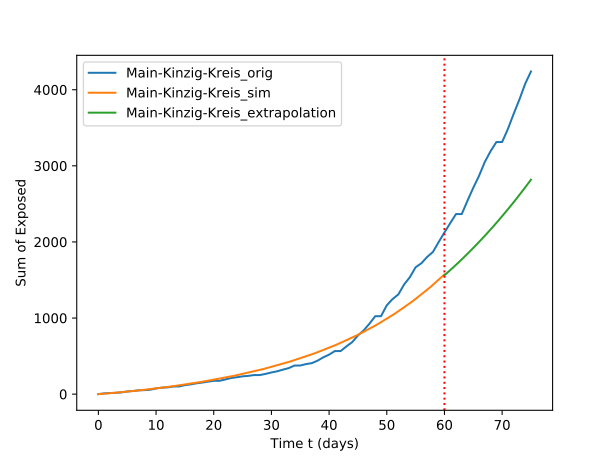
\includegraphics[width=\textwidth]{./figures/60d/13_Main-Kinzig-Kreis.png}	
		\caption{}
	\end{subfigure}
	\hfill
	\begin{subfigure}[b]{0.3\textwidth}
		\centering
		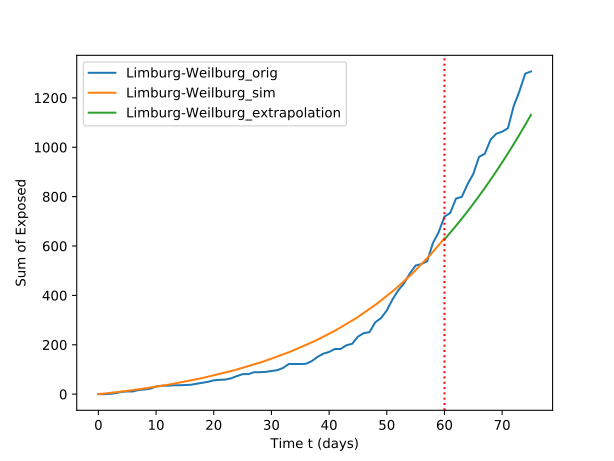
\includegraphics[width=\textwidth]{./figures/60d/10_Limburg-Weilburg.png}	
		\caption{}
	\end{subfigure}
	\begin{subfigure}[b]{0.3\textwidth}
		\centering
		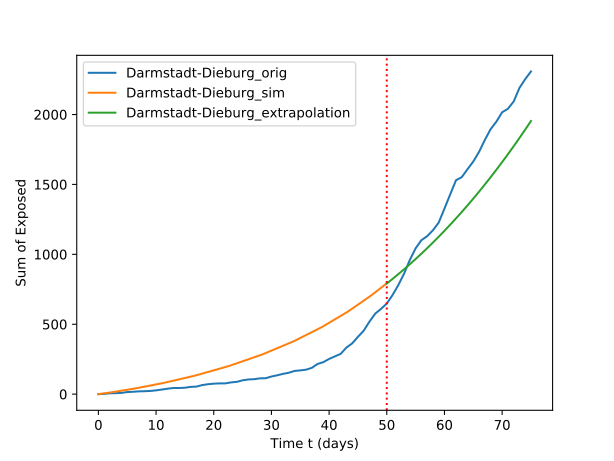
\includegraphics[width=\textwidth]{./figures/50d/24_Darmstadt-Dieburg.png}	
		\caption{}
	\end{subfigure}
	\hfill
	\begin{subfigure}[b]{0.3\textwidth}
		\centering
		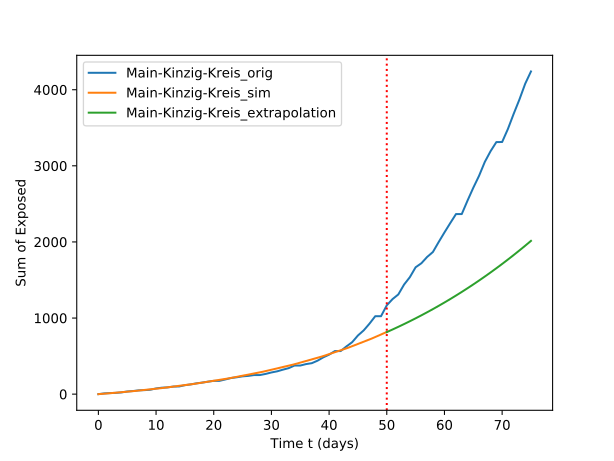
\includegraphics[width=\textwidth]{./figures/50d/13_Main-Kinzig-Kreis.png}	
		\caption{}
	\end{subfigure}
	\hfill
	\begin{subfigure}[b]{0.3\textwidth}
		\centering
		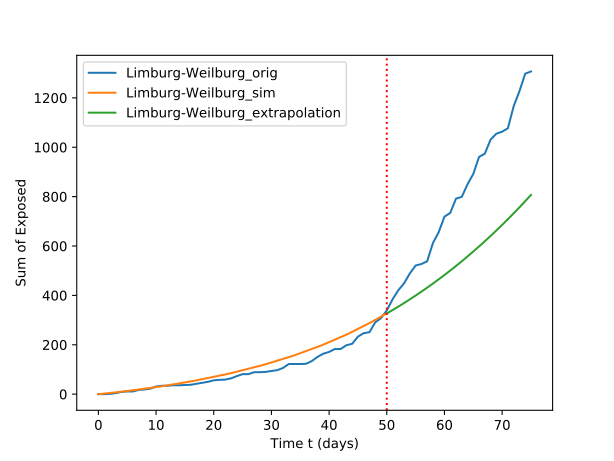
\includegraphics[width=\textwidth]{./figures/50d/10_Limburg-Weilburg.png}	
		\caption{}
	\end{subfigure}
	\caption{Three exemplary region results of the simulations of susceptible individuals. Graphs A-C, D-F and G-I
		show the results of the 76, 60 and 50 data point simulations respectively.
		The original data is drawn in blue and the simulated data is drawn in orange. In case
		of the 60 and 50 data point simulations, a red doted line marks the end of the simulated data points
		and a green line draws the extrapolated part (``extrapolation'') of the curve.
		Extrapolation was done using a third degree polynomial curve fit.
		}
	\label{fig:76_sim_expl}
\end{figure}

The figure shows, that as the number of simulated data points decreases, the trends of the simulation results shift towards
fewer transition events. This phenomenon is observable in all three regions.


%-----------------------------------
%	SUBSECTION 2
%-----------------------------------

\subsection{Deviation of the simulated data relative to the original data}
Next we analyzed the percentage deviation of the simulated data relative to the original data. This was done
for each time step in each region. The results are shown in \hyperref[fig:sim_box_sum]{figure \ref*{fig:sim_box_sum}}.
``Werra-Meissner-Kreis'', ``Marburg-Biedenkopf'' and ``Limburg-Weilburg'' are listed separately in each data set.
This was done in order to increase the plot readability, since those three regions show disproportional large deviations compared
to the other regions.\newline

\begin{figure}
	\centering
	\begin{subfigure}[b]{0.32\textwidth}
		\centering
		\caption*{\B{76 data points}}
		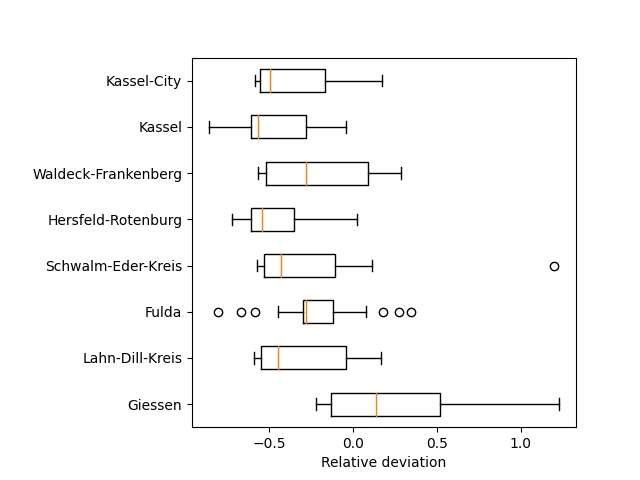
\includegraphics[width=\textwidth]{./figures/76d/deviation_box76_1.png}	
		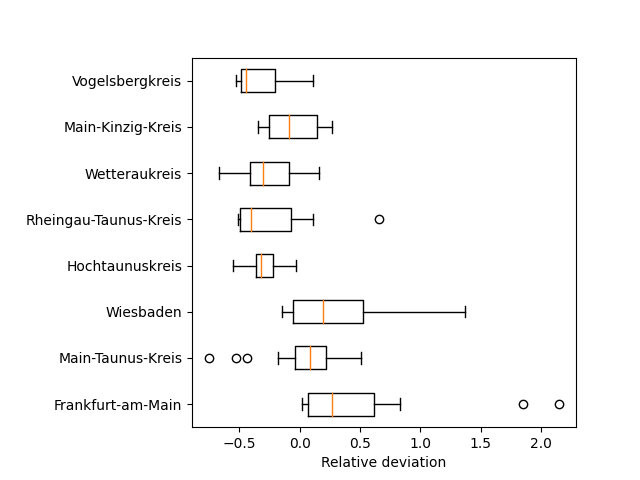
\includegraphics[width=\textwidth]{./figures/76d/deviation_box76_2.png}	
		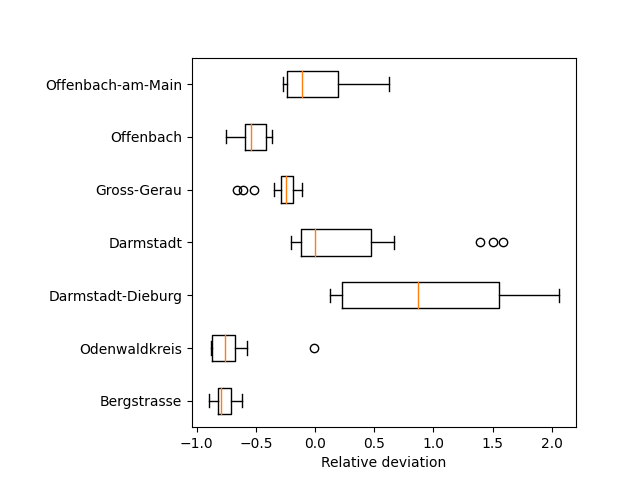
\includegraphics[width=\textwidth]{./figures/76d/deviation_box76_3.png}	
		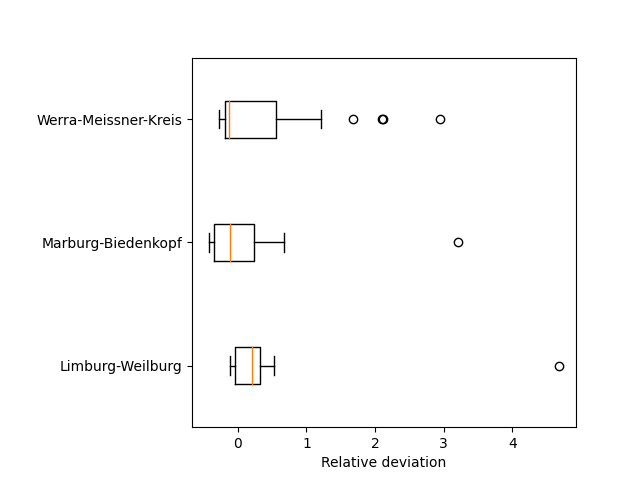
\includegraphics[width=\textwidth]{./figures/76d/deviation_box76_4.png}	
	\end{subfigure}
	\begin{subfigure}[b]{0.32\textwidth}
		\centering
		\caption*{\B{60 data points}}
		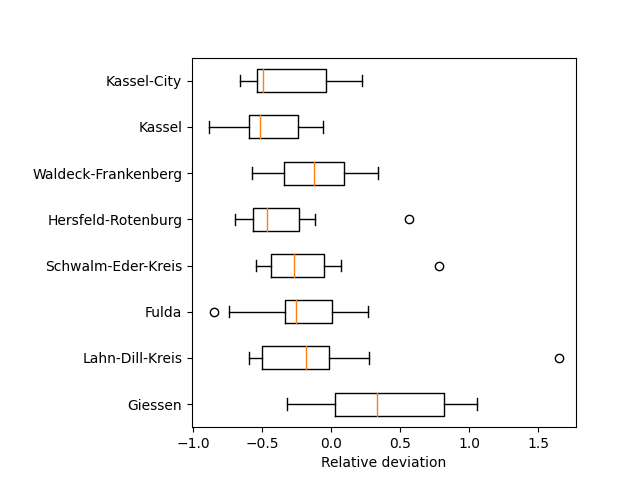
\includegraphics[width=\textwidth]{./figures/60d/deviation_box60_1.png}	
		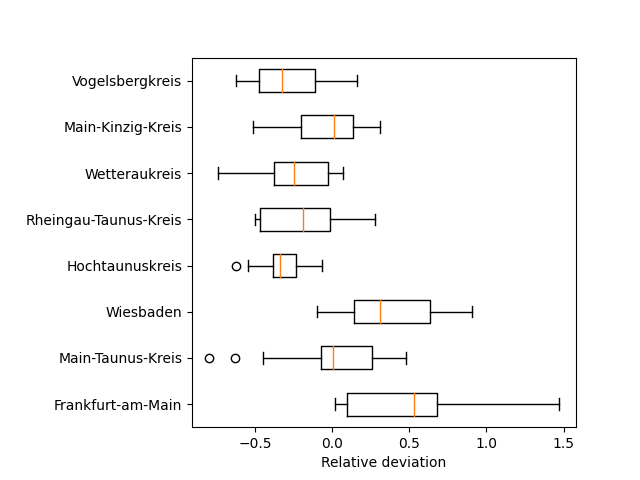
\includegraphics[width=\textwidth]{./figures/60d/deviation_box60_2.png}	
		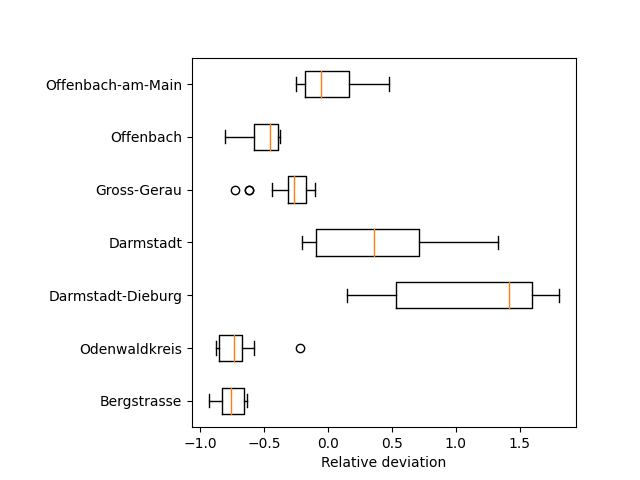
\includegraphics[width=\textwidth]{./figures/60d/deviation_box60_3.png}	
		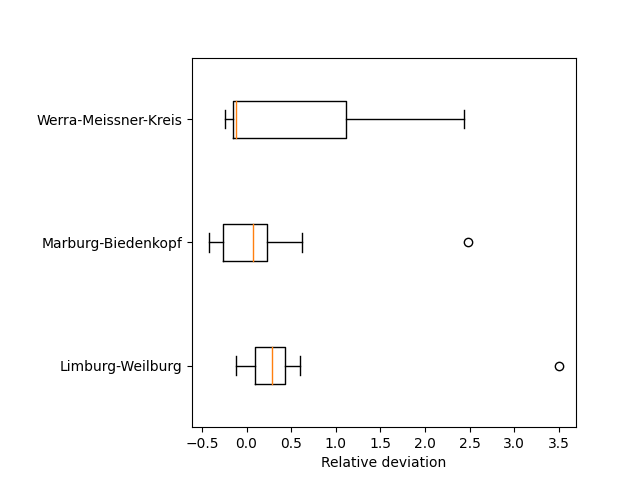
\includegraphics[width=\textwidth]{./figures/60d/deviation_box60_4.png}	
	\end{subfigure}
	\begin{subfigure}[b]{0.32\textwidth}
		\centering
		\caption*{\B{50 data points}}
		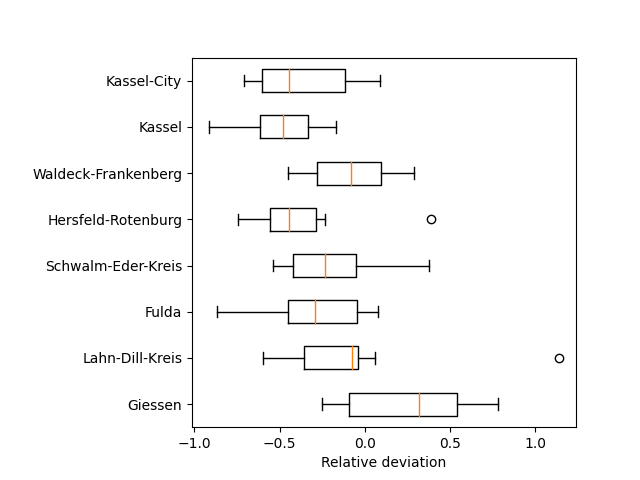
\includegraphics[width=\textwidth]{./figures/50d/deviation_box50_1.png}	
		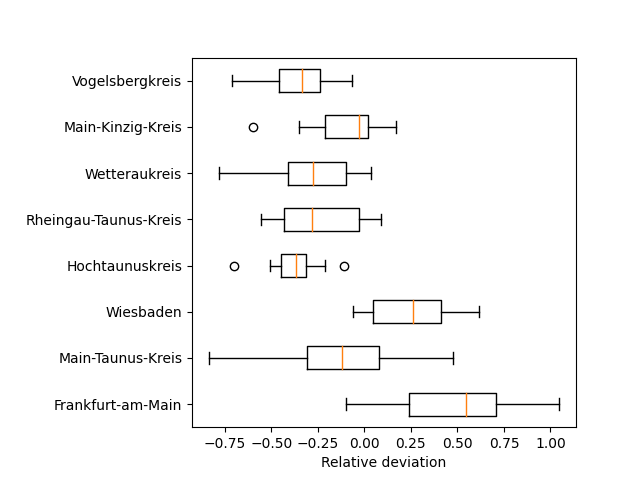
\includegraphics[width=\textwidth]{./figures/50d/deviation_box50_2.png}	
		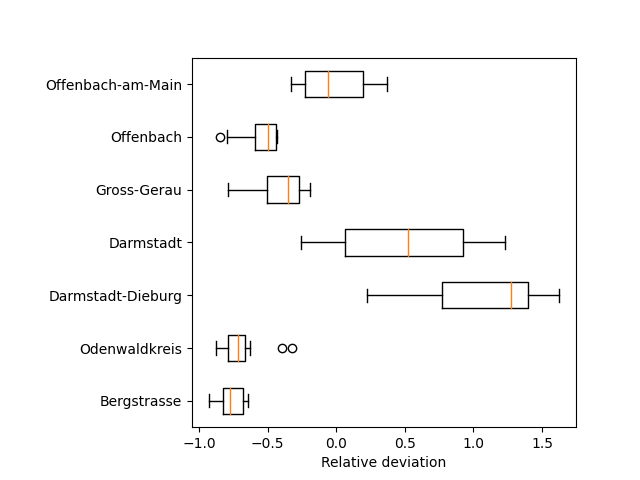
\includegraphics[width=\textwidth]{./figures/50d/deviation_box50_3.png}	
		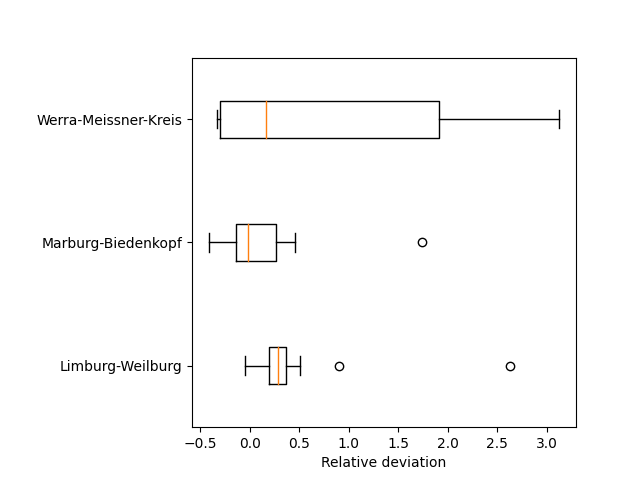
\includegraphics[width=\textwidth]{./figures/50d/deviation_box50_4.png}	
	\end{subfigure}
	\caption{Shown are box plots of the percentage deviation of every simulated region relative to the original data.
		The first column shows the box plots of the 76 data point simulations, the second and third column show
		the plots for the 60 and 50 data point simulations respectively.}
	\label{fig:sim_box_sum}
\end{figure}

All three figures show largely comparable results. Both median positions and interquartile ranges (\B{IQR}) of the regions
are mostly similar across all three simulations. Differences can mostly be observed regarding the Minimum and Maximum of different regions
and the skew of the individual regions. In the 76 data point data set most of the regions show the median in the left
part of the \B{IQR}, meaning the plot is skewed right. This however changes in the other two simulations, with medians
shifting more to the right in the 60 and even more so in the 50 data point simulations. \hyperref[tab:box_sum]{Table \ref*{tab:box_sum}}
summarizes additional information about the different data sets. \hyperref[tab:optimized_var]{Table \ref*{tab:optimized_var}}
shows the optimal values for $\alpha$ and $q$ that were determined by the optimization procedure of the model.
\textcolor{red}{add data to Appendix!!!}

\begin{table}
	\centering
	\caption{Summary of statistical data regarding the box plots shown in figure \ref*{fig:sim_box_sum}.
		Abbreviations used include Number of regions (\B{\#Regions}), median deviation (\B{MD})}
	\begin{tabular}{|l||c|c|c|}
		\hline
		Simulated data set & 76 data points & 60 data points & 50 data points \\ \hline \hline
		Minimum \B{MD} & -0.792 & -0.757 & -0.772 \\ \hline
		Maximum \B{MD} & 0.868 & 1.418 & -1.275 \\ \hline
		\B{\#Regions} with absolute \B{MD} $< 0.25$ & 10 & 9 & 8 \\ \hline
		\B{\#Regions} with absolute \B{MD} $< 0.50$ & 20 & 21 & 21 \\ \hline
		\B{\#Regions} with absolute \B{MD} $< 0.75$ & 23 & 24 & 24 \\ \hline
		\B{\#Regions} with MD $<0$ & 19 & 17 & 19 \\ \hline
		\B{\#Regions} with MD $\geq 0$ & 7 & 9 & 7 \\ \hline
	\end{tabular}
	\label{tab:box_sum}
\end{table}

\begin{table}
	\centering
	\caption{Best values obtained for $\alpha$ and $q$. The values were determined during the optimization process
		using \I{ConstrainedOptimization}.}
	\begin{tabular}{|l||c|c|c|}
		\hline
		Simulated data set & 76 data points & 60 data points & 50 data points \\ \hline \hline
		optimal $\alpha$ & 0.1975 & 0.1974 & 0.1920\\ \hline
		optimal $q$ & 6.6753 & 6.6749 & 6.6750 \\ \hline
	\end{tabular}
	\label{tab:optimized_var}
\end{table}

%----------------------------------------------------------------------------------------
%	SECTION 2
%----------------------------------------------------------------------------------------

\section{Influence of individual regions on the loss function}
\textcolor{red}{add table with total information to Appendix}
In order to better understand the influence of individual regions on the model itself, we manually calculated the total
loss, the loss for each individual region and the percentage loss of each region relative to the total loss. The
calculation was done using the final output data of the 76 data point simulation.
\hyperref[tab:perc_region_loss]{Table \ref*{tab:perc_region_loss}} shows the percentage of the total loss each region
has and compares it to the percentage population the region has relative to the total population. The percentage
of the total loss a region has is proportional to its influence on the variable optimization process.
The table is sorted in descending order from highest percentage loss contribution to lowest.\newline

\begin{table}[h]
	\caption{Influence of the }
	\centering
	\begin{tabular}{|l|x{2cm}|x{2cm}|x{2cm}|}
	%\begin{tabular}{|l|c|c|c|}
		\hline
		\B{region} & \B{percentage loss} & \B{percentage population} & \B{median deviation} \\ \hline \hline
		Offenbach & 27.70 & 5.67 & -0.545 \\ \hline
		Bergstrasse & 14.41 & 4.31 & -0.792 \\ \hline
		Frankfurt-am-Main & 13.10 & 12.14 & 0.270 \\ \hline
		Lahn-Dill-Kreis & 6.29 & 4.03 & -0.448 \\ \hline
		Main-Kinzig-Kreis & 5.17 & 6.70 & -0.093 \\ \hline
		Marburg-Biedenkopf & 4.70 & 3.91 & -0.106 \\ \hline
		Kassel-City & 3.90 & 3.19 & -0.494 \\ \hline
		Wetteraukreis & 3.35 & 4.93 & -0.304 \\ \hline
		Gross-Gerau & 2.90 & 4.38 & -0.244 \\ \hline
		Rheingau-Taunus-Kreis & 2.89 & 2.98 & -0.402 \\ \hline
		Kassel & 2.58 & 3.77 & -0.565 \\ \hline
		Hochtaunuskreis & 2.33 & 3.77 & -0.320 \\ \hline
		Darmstadt-Dieburg & 2.00 & 4.73 & 0.868 \\ \hline
		Odenwaldkreis & 1.93 & 1.54 & -0.759 \\ \hline
		Offenbach-am-Main & 1.23 & 2.08 & -0.108 \\ \hline
		Schwalm-Eder-Kreis & 1.03 & 2.86 & -0.430 \\ \hline
		Waldeck-Frankenberg & 0.99 & 2.49 & -0.283 \\ \hline
		Giessen & 0.84 & 4.32 & 0.137 \\ \hline
		Wiesbaden & 0.80 & 4.43 & 0.194 \\ \hline
		Fulda & 0.74 & 3.54 & -0.281 \\ \hline
		Hersfeld-Rotenburg & 0.41 & 1.91 & -0.545 \\ \hline
		Main-Taunus-Kreis & 0.25 & 3.80 & 0.083 \\ \hline
		Darmstadt & 0.18 & 2.53 & 0.002 \\ \hline
		Vogelsbergkreis & 0.17 & 1.68 & -0.442 \\ \hline
		Limburg-Weilburg & 0.08 & 2.74 & 0.211 \\ \hline
		Werra-Meissner-Kreis & 0.03 & 1.59 & -0.123 \\ \hline
	\end{tabular}
	\label{tab:perc_region_loss}
\end{table}

The results show, that a minority of regions contribute to the majority of the total loss in the model. The top three contributors
account for 55.21 percent of the entire loss, while only making up about 22.12 percent of the total population. The top seven
contributors make up about 75.27 percent, while making up about 39.95 percent of the population. A notable find is, that the
top two regions, ``Offenbach'' and ``Bergstrasse'', both display a negative deviation, while the third most influential region
``Frankfurt-am-Main'' has a positive deviation. Frankfurt also has a lower overall contribution to the loss, than the other
two regions, even though it has a higher share of the total population than the other two regions combined.

%----------------------------------------------------------------------------------------
%	SECTION 3
%----------------------------------------------------------------------------------------

\section{Sensitivity analysis of $\alpha$ and $q$}
In order to further investigate the features of the model, we analyzed the sensitivity of the loss function relative to
the variables $\alpha$ and $q$. 4000 simulations of the model with all 76 original data points were performed and the variables
$\alpha$ and $q$ were chosen randomly, within a set constraint. The upper and lower bounds were set from 0.05 to 0.35 for 
$\alpha$ and 5.5 to 8.0 for $q$ respectively. These ranges were chosen based on the optimized values of the previous
experiments. The results of these simulations were gathered and $\alpha$, $q$ and the loss were  plotted against one another.
The result is a topographic map of the variable landscape of the loss of the susceptible group.
\hyperref[fig:sensitivity_zoom0]{Figure \ref*{fig:sensitivity_zoom0}} shows the total result of all simulations over the chosen bounds.
Each point plotted is color coded, relative to the maximum loss of all values displayed. Points with a higher loss are colored red,
while plots with lower loss are colored green.

\begin{figure}[h]
	\centering
	\begin{subfigure}[b]{0.4\textwidth}
		\centering
		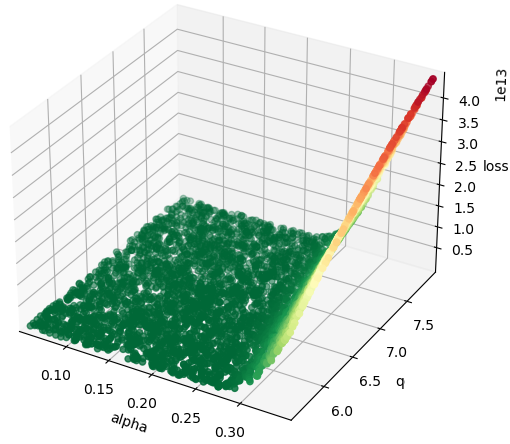
\includegraphics[width=\textwidth]{./figures/sensitivity/sensitivity_zoom0_0_2.png}	
		\caption{}
	\end{subfigure}
	\begin{subfigure}[b]{0.4\textwidth}
		\centering
		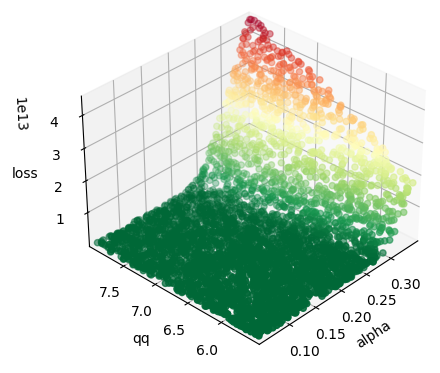
\includegraphics[width=\textwidth]{./figures/sensitivity/sensitivity_zoom0_1_2.png}	
		\caption{}
	\end{subfigure}
	\caption{Visualization of the variable sensitivity of the susceptible group. The variables $\alpha$ and $q$ were plotted
		against the loss of the susceptible group. Images (A) and (B) show the plot from different angles in order
		to increase readability. In the model the susceptible group shows sensitivity to changes of both $\alpha$ and
		$q$. However, the sensitivity to $q$ seems to be dependent on $\alpha$.
		}
	\label{fig:sensitivity_zoom0}
\end{figure}

Figure \ref*{fig:sensitivity_zoom0} shows that low values for $\alpha$ cause a low sensitivity of the model
for $q$. After an $\alpha$ value of about 0.25 is reached, the loss value starts to react to changes in $q$. Further
increases of $\alpha$ or $q$, cause the loss function increases quickly. Changes in $\alpha$ appear to have a bigger effect
on the loss, but a bigger $q$ value causes the loss to increase more quickly compared to a simulation with a smaller $q$.\newline

The simulations were further investigated by plotting only part of the experimental data.
The first row of \hyperref[fig:sensitivity_zoom1]{Figure \ref*{fig:sensitivity_zoom1}} shows all data points with $\alpha$ values between 0.15
and 0.25, $q$ values between 5.5 and 8.0 and a maximum loss of $10^{10}$. The loss on this image was capped in order to reduce
the scale of the loss and thereby increase readability. This lead to 957 of 4000 data points being plotted. The images in the
second row show the same graph, but with a maximum loss capped at $2.7*10^{9}$.

\begin{figure}[h]
	\centering
	\begin{subfigure}[b]{0.4\textwidth}
		\centering
		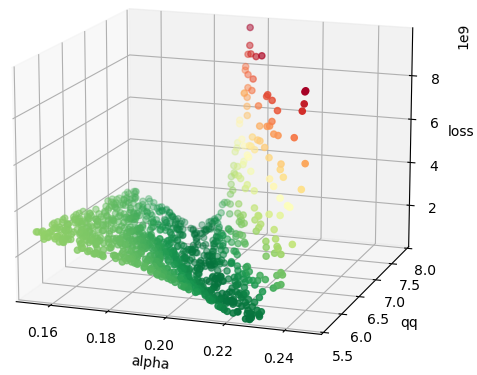
\includegraphics[width=\textwidth]{./figures/sensitivity/sensitivity_zoom1_0_2.png}	
	\end{subfigure}
	\begin{subfigure}[b]{0.4\textwidth}
		\centering
		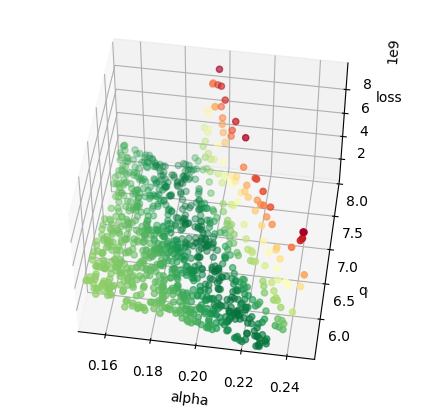
\includegraphics[width=\textwidth]{./figures/sensitivity/sensitivity_zoom1_1_2.png}	
	\end{subfigure}
	\begin{subfigure}[b]{0.4\textwidth}
		\centering
		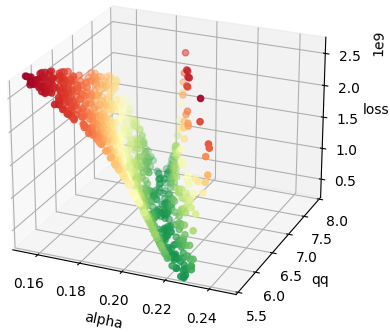
\includegraphics[width=\textwidth]{./figures/sensitivity/sensitivity_zoom2_0_2.png}	
	\end{subfigure}
	\begin{subfigure}[b]{0.4\textwidth}
		\centering
		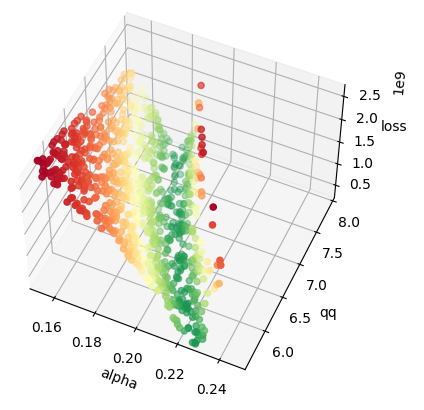
\includegraphics[width=\textwidth]{./figures/sensitivity/sensitivity_zoom2_1_2.png}	
	\end{subfigure}
	\caption{Visualization of the variable sensitivity of the susceptible group. The variables $\alpha$ and $q$ were
		capped to 0.15 and 0.25 and 5.5 and 8.0 respectively and then plotted against the result of the loss function.
		The loss was capped at $10^{10}$ and $2.7*10^{9}$ for the first and the second row respectively, in order to
		reduce the scale of the loss and make the image more readable. The image shows that there seems to be a set of
		optimal value combinations of $\alpha$ and $q$, where the loss is minimized. Given the diagonal nature of this
		``optimal cavity'' there seem to be an equilibrium between the two values.
		\textcolor{red}{check for better wording} %note
		}
	\label{fig:sensitivity_zoom1}
\end{figure}

Figure \ref*{fig:sensitivity_zoom1} shows the existence of a ``valley'' with minimized loss. It can be seen that there are 
sets of values of $\alpha$ and $q$, where the loss appears to be minimized. The optimal values found by the model for $\alpha$
(0.1975) and $q$ (6.6753) are also within this region. The optimized area seems to have a diagonal structure,
indicating an optimal relation between $\alpha$ and $q$.

